%\documentclass[11pt,a4paper]{report}


% The Beamer class comes with a number of default slide themes
% which change the colors and layouts of slides. Below this is a list
% of all the themes, uncomment each in turn to see what they look like.

%\usetheme{default}
%\usetheme{AnnArbor}
%\usetheme{Antibes}
%\usetheme{Bergen}
%\usetheme{Berkeley}
%\usetheme{Berlin}
%\usetheme{Boadilla}
%\usetheme{CambridgeUS}
%\usetheme{Copenhagen}
%\usetheme{Darmstadt}
%\usetheme{Dresden}
%\usetheme{Frankfurt}
%\usetheme{Goettingen}
%\usetheme{Hannover}
%\usetheme{Ilmenau}
%\usetheme{JuanLesPins}
%\usetheme{Luebeck}
%\usetheme{Madrid}
%\usetheme{Malmoe}
%\usetheme{Marburg}
%\usetheme{Montpellier}
%\usetheme{PaloAlto}
%\usetheme{Pittsburgh}
%\usetheme{Rochester}
%\usetheme{Singapore}
%\usetheme{Szeged}
%\usetheme{Warsaw}

\documentclass[10pt]{beamer}
\usepackage{float}
\usepackage[nodisplayskipstretch]{setspace}
\usepackage{pdfpages}
\usepackage{tikz}    
\usetheme{metropolis}
\usepackage{appendixnumberbeamer}
\usepackage[normalem]{ulem}
\usepackage{eurosym}
\usepackage{booktabs}
\usepackage[scale=2]{ccicons}
\usepackage[utf8]{inputenc}
\usepackage{soul}
\usepackage{mathabx}
\usepackage{graphicx}
\usepackage{pgfplots}
\usepgfplotslibrary{dateplot}
 \usepackage{relsize}
\usepackage{xspace}
\usepackage{caption}

\usepackage{graphicx}
\usepackage{graphicx}

\usepackage{hyperref}
\hypersetup{
    colorlinks=true,
    linkcolor=blue,
    filecolor=magenta,      
    urlcolor=blue,
}
 
\urlstyle{same}
\newcommand{\themename}{\textbf{\textsc{metropolis}}\xspace}


% As well as themes, the Beamer class has a number of color themes
% for any slide theme. Uncomment each of these in turn to see how it
% changes the colors of your current slide theme.

%\usecolortheme{albatross}
%\usecolortheme{beaver}
%\usecolortheme{beetle}
%\usecolortheme{crane}
%\usecolortheme{dolphin}
%\usecolortheme{dove}
%\usecolortheme{fly}
%\usecolortheme{lily}
%\usecolortheme{orchid}
%\usecolortheme{rose}
%\usecolortheme{seagull}
%\usecolortheme{seahorse}
%\usecolortheme{whale}
%\usecolortheme{wolverine}

%\setbeamertemplate{footline} % To remove the footer line in all slides uncomment this line
%\setbeamertemplate{footline}[page number] % To replace the footer line in all slides with a simple slide count uncomment this line

%\setbeamertemplate{navigation symbols}{} % To remove the navigation symbols from the bottom of all slides uncomment this line


\usepackage[utf8]{inputenc}
\usepackage{graphicx}

\usepackage{amsmath,amsthm,amssymb,latexsym,amsfonts}


\setlength{\parindent}{15pt}
\usepackage{subfig}
\usepackage{hyperref}
\usepackage{graphicx} % Allows including images
\usepackage{booktabs} % Allows the use of \toprule, \midrule and \bottomrule in tables
\usepackage{braket}
\usepackage{amsmath}
\usepackage[makeroom]{cancel}

\usepackage{bm}

%\title{Probar que un predicado es primitivo recursivo sin marearse}
%\author{Guillermo Mosse}


%TODO todo el tiempo preguntar si hay preguntas!


\begin{document}
%TODO cambiar rojo y azul por colores que tenga marcador. No, cnseguir uno azul para pizarron

% Llego y divido el pizarrón en 2
% Hola, qué tal? Elegí contar el ejercicio de la materia Lógica y Computabilidad, que pide probar que cierto predicado es primitivo recursivo. Voy a presentar el ejercicio, su contexto, su resolución, y al final voy a dejar un par de enunciados parecidos para mis...alumnos imaginarios.

\title{Constraint Normalization and Parameterized Caching for Quantitative Program Analysis, por }
\subtitle{Tegan Brennan, Nestan Tsiskaridze, Nicolás Rosner, Abdulbaki Aydin, y Tevfik Bultan\\\tiny{LIA significa Linear Integer Arithmetic}}
% \date{\today}
\date{}
\author{Guillermo Mosse}

\maketitle


\begin{frame}{Contexto y Motivación}
%TODO me falta motivacion

Ejemplo de constraint: $\{(x,y) \in \mathbb{Z}^2 : y = 2 \land 4 \geq x \geq y\}$

Otro ejemplo: $\{ (a,b,e) : a = "@" \land b = ".com" \land suffix\_of(b,e) \land contains(a,e)\}$

Pueden aparecer como path constraints al hacer symbolic execution de programas que manipulen strings, como por ejemplo:
\begin{itemize}
	\item Generadores de queries para bases de datos
	\item Generadores dinámicos de código
	\item Validadores de inputs en aplicaciones web
\end{itemize} \pause

¿Qué se puede querer al trabajar con constraints?

\begin{itemize}
	\item Satisfiability.
	\item Solution set.
	\item Model counting (y bounded model counting).
\end{itemize}

¡Todas son muy costosas! (¿Satisfiability también?)
	
\end{frame}

\begin{frame}{Contribuciones del paper}
\begin{itemize}
	\item Se dieron cuenta de que en model counting dos constraints escritas de manera distinta pueden ser equivalentes, i.e., expresan lo mismo.
	\item Diseñaron e implementaron una manera poco costosa de ver cuándo dos constraints son equivalentes: ver si sus formas normales son iguales
	\item Implementaron el algoritmo que computa la forma normal
	\item Hicieron un experimento cacheando soluciones y mostraron que mejora los tiempos.
\end{itemize}
\end{frame}



\begin{frame}{La idea del paper: hecho con KolourPaint}
\begin{figure}[H]
\centering
    \includegraphics[scale=0.6]{plot1.png}
    \captionsetup{labelformat=empty}
    \caption{Mi universo de constraints\\(tengan imaginación)}
\end{figure}
\end{frame}

\begin{frame}{La idea del paper}
\begin{figure}[H]
\centering
    \includegraphics[scale=0.6]{plot2.png}
    \captionsetup{labelformat=empty}
    \caption{Defino cuándo son equivalentes (pero es muy costoso responder cuando una constraint es equivalente a otra)} %"Ir probando" es imposible. Decir que el conjunto C = {d: d constraint equivalente a c} podría llegar a ser c.e. en un conjunto más general. Decir que se puede ir probando y etcétera.
\end{figure}
\end{frame}

\begin{frame}{La idea del paper}
\begin{figure}[H]
\centering
    \includegraphics[scale=0.6]{plot3.png}
    \captionsetup{labelformat=empty}
    \caption{Es más fácil trabajar con una relación de orden\\(¡puedo navegar por el grafo más fácil!)}
\end{figure}
\end{frame}

\begin{frame}{La idea del paper}
\begin{figure}[H]
\centering
    \includegraphics[scale=0.6]{plot4.png}
    \captionsetup{labelformat=empty}
    \caption{La forma normal es bajar hasta no poder más, y es única\\Para comparar dos constraints computo su forma normal y me fijo si son iguales}
\end{figure}
\end{frame}

% Algo interesante es que el paper es redundante
% No lei muchos papers de matematica en mi vida
% Pero no suelen ser redundantes
% Igual estoy super a favor de la redundancia
% Me encanta que un paper sea redundante

\begin{frame}{¿Cómo son las constraints?}


\begin{figure}[H]
\centering
    \includegraphics[scale=0.6]{figure2.png}
    \captionsetup{labelformat=empty}
    \caption{Definimos los términos de tipo String, Reg Exp y Aritmético}
\end{figure}
\end{frame}

\begin{frame}{¿Cómo son las constraints?}
\begin{figure}[H]
\centering
    \includegraphics[scale=0.6]{figure3.png}
    \captionsetup{labelformat=empty}
    \caption{El lenguaje L tiene conjuncts de tipo String, Reg Exp, y Aritméticos.}
\end{figure}
\end{frame}

\begin{frame}{¿Cómo son las constraints?}
\begin{figure}[H]
\centering
    \includegraphics[scale=0.6]{figure2.png}
    \captionsetup{labelformat=empty}
\end{figure}
\begin{figure}[H]
\centering
    \includegraphics[scale=0.6]{figure3.png}
    \captionsetup{labelformat=empty}
\end{figure}

\end{frame}


%% en el algoritmo 4 no tienen en cuenta el bound!!!!
%% tenerlo en cuenta te obliga a cambiar el algoritmo porque en el fondo es una conjuncion de mas condiciones (tantas como variables aparezcan)
\begin{frame}{\textbf{Bounded} model counting}
Una aclaración: algo que no incluye lo anterior es que podemos pedir que las constraints vengan con un bound $b$ que fije un máximo para el tamaño de las soluciones (sean ints o strings). Por ahora ignorémoslo.

%TODO DIEGO: section 3 al final: no entiendo lo del hit/miss...quiero chequear con el el Algorithm 1

%TODO DIEGO: hay bounds para longitud de strings? creo que si

%TODO section 4 en el medio....por que sirve tambien cuando hay que tener el solution set? y que cambia si solo hay que saber si se satisface o no? como cambia la normalizacion?

\end{frame}

\begin{frame}{¿Cuándo dos constraints son equivalentes?}


Ejemplo:

$$c_1 := \{(x,y) \in \mathbb{Z}^2 : y = 2 \land y \leq x\ \leq 4\}$$
Soluciones: $\{(2,2); (2,3) ; (2,4)\}$

\textbf{es equivalente a:}

$$c_1 := \{(x,y) \in \mathbb{Z}^2 : y = 3 \land y \leq x \leq 5\}$$
Soluciones: $\{(3,3); (3,4) ; (3,5)\}$


\textbf{porque ambas tienen 3 soluciones...?} \pause

Y qué pasa con:

$c_3 := \{(x,y) \in \mathbb{Z}^2 : 0<=x<=1 \land y = 3\}$\\$c_4 := \{(x) \in \mathbb{Z}^2 : 0<=x<=1\}$ \pause

Definir así la relación de equivalencia es muy poco manejable. ¿Por qué?
% Piensen que cashew va a tener que responder cuándo dos constraints son equivalentes
% ¡no queremos que para responder eso tenga que evaluar la cantidad de soluciones que tenga cada constraint!
% necesitamos reglas sintácticas para decidir cuándo dos constraints son equivalentes
\end{frame}


\begin{frame}{¿Cuándo dos constraints son equivalentes?}

Dos constraints van a ser equivalentes cuando pueda llegar de una a la otra.

¿De qué manera?

Por medio de unas "transformaciones de constraints" que \textbf{siempre} mantienen la cardinalidad de las soluciones, \textbf{tengo definidas explícitamente}, y representan una transformación \textbf{sintáctica}.

¿Qué transformaciones de constraints siempre mantienen la cardinalidad?
\end{frame}

\begin{frame}{Transformaciones de constraints: construyamos $\mathbb{G}_{card}$}
%Pensemos primero en transformaciones de conjuncts (constraints con una sola condición):
\begin{itemize}
	\item Puedo cambiar el nombre de las variables para strings e ints.
	\item Puedo cambiar el orden de las condiciones separadas por ANDs.
	\item Puedo permutar los elementos del alfabeto $\Sigma$ que se usa para los strings.\pause
	\item Si veo a una constraint como un \textbf{conjunto de puntos en el espacio}...\\¿rotaciones? ¿traslaciones? ¿simetrías?


\begin{figure}[H]
\centering
    \includegraphics[scale=0.3]{rotation.png}
    \includegraphics[scale=0.3]{traslation.png}
    \includegraphics[scale=0.3]{symmetry.png}
    \captionsetup{labelformat=empty}
\end{figure} \pause

¿Cuántas transformaciones hay?

¿Estas transformaciones definen la misma relación de equivalencia que la primera idea de "dos conjuntos son equivalentes si tienen la misma cantidad de soluciones"?


	
\end{itemize}

%las rotaciones y simetrias no andan porque tienen que actuar sobre todos los conjuntos
%\includegraphics[scale=0.3]{rotation.png} \\
%\includegraphics[scale=0.3]{traslation.png} \\
%\includegraphics[scale=0.3]{symmetry.png}

\end{frame}

\begin{frame}{¡Es un grupo!}

¡Las transformaciones forman un grupo!

O sea:

\begin{itemize}
	\item Hay una operación que se le puede hacer a dos transformaciones: \textbf{componerlas}
	\item Hay un elemento que es "el neutro": la identidad (dejar las constraints tal como están)
	%Observar que la identidad compuesta con otra transformacion es otra transformacion
	\item Toda transformación tiene un inverso: "deshacer el cambio".
\end{itemize}

%TODO contar que es un producto cartesiano de grupos también
\end{frame}

\begin{frame}{Esperen, ¡aun hay más!}

Más aun, es un producto cartesiano de 4 grupos más manejables todavía.

Dada $g \in \mathbb{G}_{card}$, ésta se puede identificar con una 4-upla formada por:
\begin{itemize}
	\item una permutación de nombres de variables.
	\item una permutación de las condiciones separadas por ANDs.
	\item una permutación de los elementos del alfabeto $\Sigma$.
	\item una traslación de la constraint:(sumar $k \in \mathbb{Z}$ a todas las constantes a la vez).
\end{itemize}

\end{frame}


\begin{frame}{Digresión sobre grupos}
Si $C$ es un conjunto y tengo un grupo $G$ que actúa sobre ese conjunto (en el sentido de antes: dado $x \in C$ y $g \in G$ puedo hacer $g(x)=y\in C$), se puede estudiar la relación de equivalencia que queda definida.

Esto es algo muy hecho en matemática y al estudiar \textbf{cómo actúa un grupo sobre un espacio} uno puede obtener \textbf{información útil} sobre ese espacio. Es más: \textbf{así es como empezó la teoría de grupos}; surgieron con los grupos de permutación, usados por Lagrange en su trabajo sobre raíces de polinomios.

%TODO completar!!!

%Dado un conjunto $C$, estudiar la acción de un grupo $G$ sobre ese conjunto es algo muy hecho en matemática.
%Más específicamente, se estudiar la relación de equivalencia definida 
\end{frame}

\begin{frame}{Digresión sobre relaciones de equivalencia}

Dada una relación de equivalencia ~ sobre un conjunto $C$ que puede o no haber venido por un grupo, dados $x,y\in C$ es en general indecidible responder si $x~y$. (O muy costoso si la relación es finita). Este paper encuentra una manera de resolver el problema, ¡pero no siempre se puede hacer eso! \pause

\end{frame}


\begin{frame}{Un ejemplo indecidible "simple"}

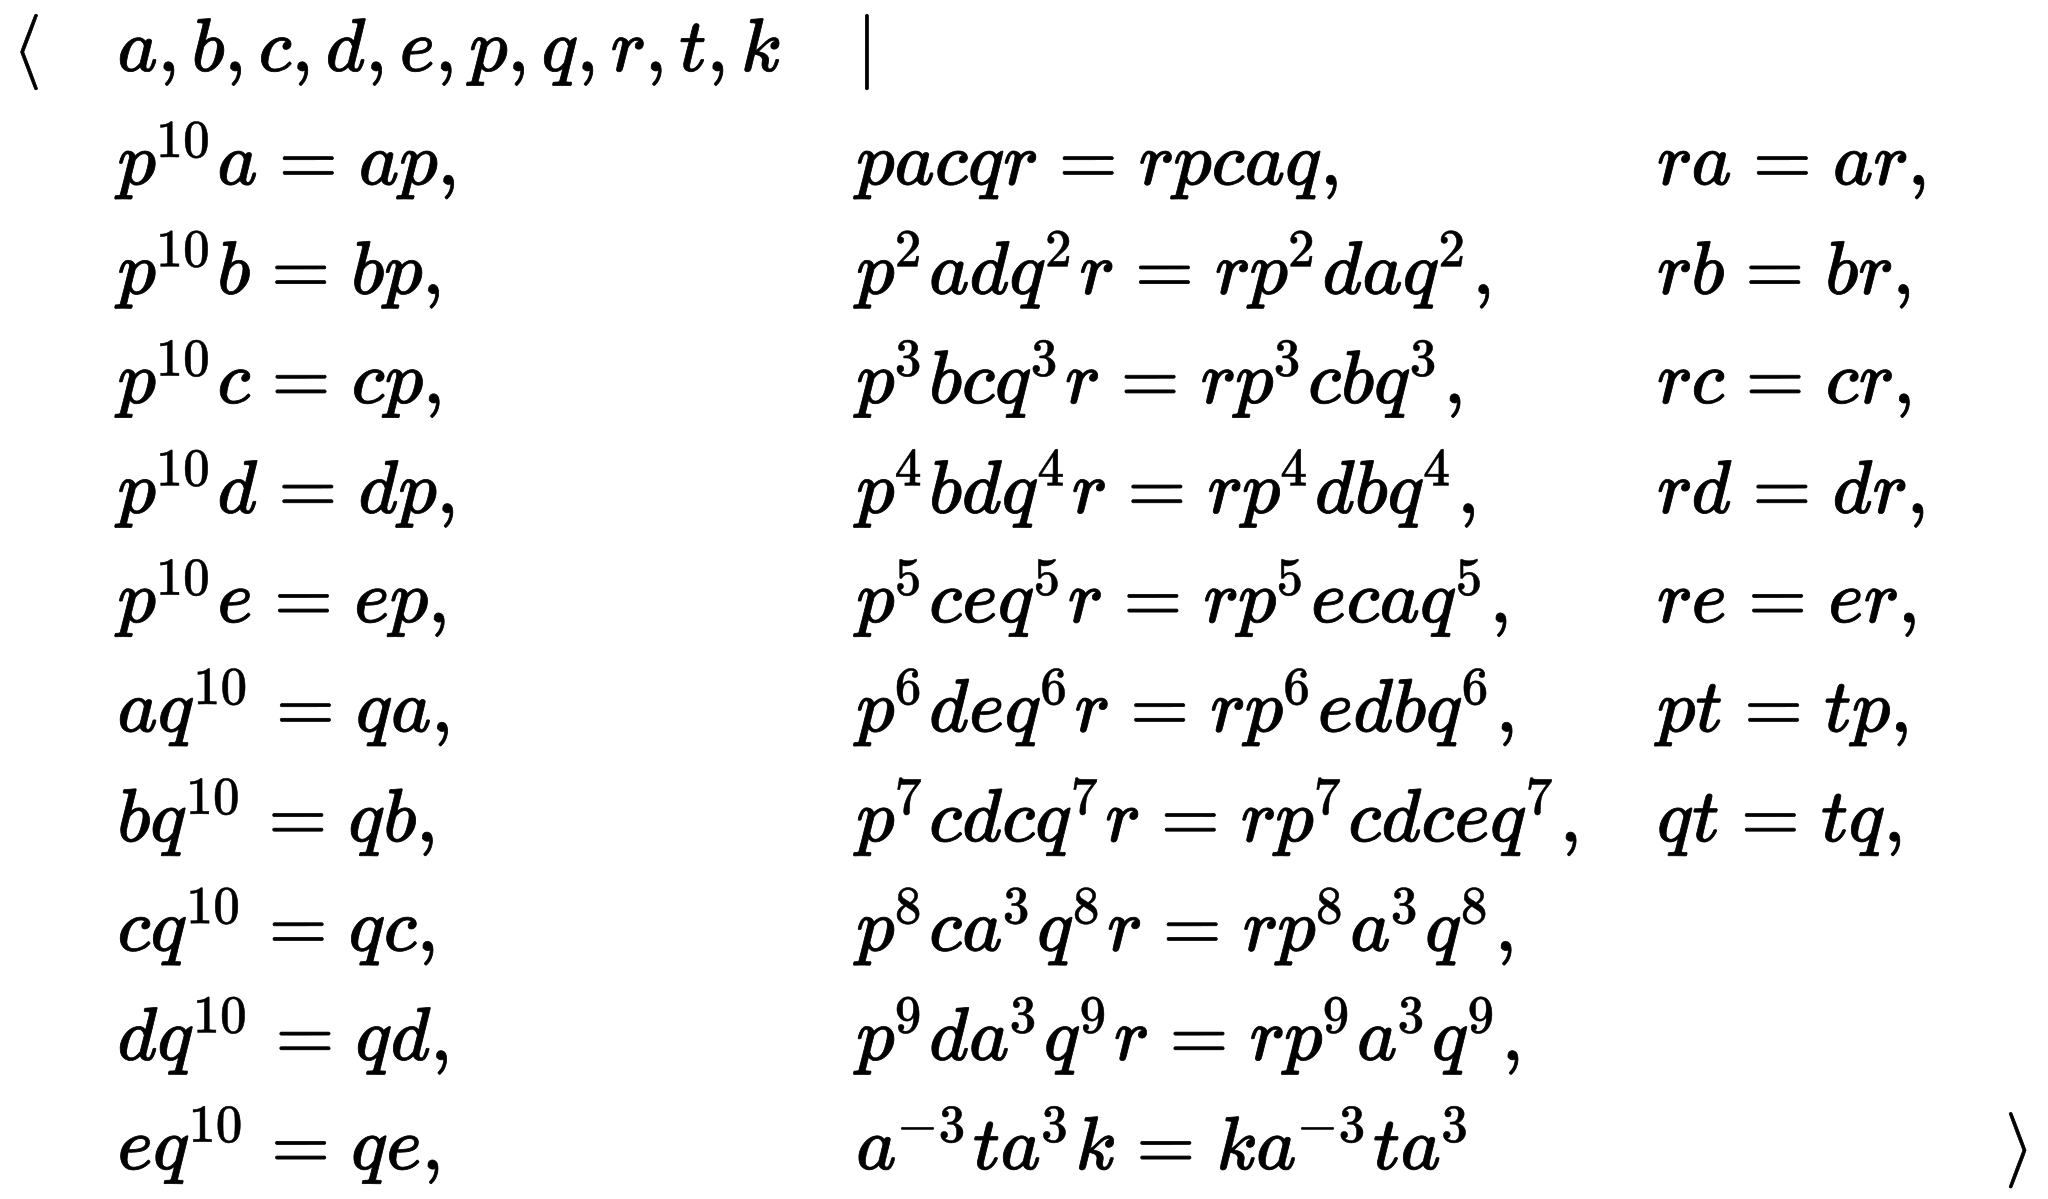
\includegraphics[scale=0.35]{unsolvable.png}

(donde las igualdades "generan" la relación de equivalencia) el word problem es indecidible.
\end{frame}


\begin{frame}{Ahora la relación de orden}
	¿Cómo transformamos la relación de equivalencia en una relación de orden? \pause
	Ordenando constraints de manera lexicográfica...o casi. \pause
	\includegraphics[scale=1]{alg2.png}
	
	Dos constraints son comparadas primero por la cantidad de conjuncts que tienen, y si el número es igual, por el primer conjunct de una que es menor que la otra.
\end{frame}

%TODO DIEGO no entiendo VI(F) que hace!!!
% en particular no entiendo lo de "relative"
% sigma(F) si que se entiende....
\begin{frame}{La relación de orden: algunos ejemplos}
\includegraphics[scale=1.5]{alg2_imp.png}
	
	$\{a : a<1\}$\visible<1>{ vs}\visible<2->{$<$}  $\{a : a<1 \land a>2\}$
	
	
	$\{a : a<1\}$\visible<1,2>{ vs}\visible<3->{$<$}$\{c : c<1\}$

		$\{a : a<5\}$\visible<1-3>{ vs}\visible<4->{$<$}$\{c : c<1\}$


	$\{(a,b) : a<2 \land b<4\}$\visible<1-4>{ vs} \visible<5->{$<$}$\{(a,b) : a<2 \land b \leq 1\}$

	$\{(s,b) : s= \text{"rana"} \land b=4\}$\visible<1-5>{ vs}\visible<6->{$>$} $\{(s,b) : s=\text{"rama"} \land b=1\}$

\end{frame}


\begin{frame}{El algoritmo}
	Una vez tenemos definida la relación de orden, podemos considerar solo las transformaciones $g$ que a una constraint la "achican".
	\includegraphics[scale=1]{ordered_descent.png}
	
	%Aplicándoselas a una constraint, como es un buen orden, después de finitas iteraciones no podemos bajar más: esa es la forma normal.
\end{frame}

\begin{frame}{El algoritmo (II)}
\includegraphics[scale=1]{alg4.png}

Observación: en la práctica, a partir de la constraint, computás el mínimo que podés obtener con las $g$ de cada subgrupo discutido.


Pregunta: ¿Por qué recorren todas las permutaciones de conjuncts?
%¿Por qué no tienen una función que sea "buscar el mínimo, o algo así? ¿Qué es lo que no anda?
\end{frame}

\begin{frame}{Uno más rápido pero que no devuelve forma normal}

\includegraphics[scale=1]{alg5.png}\\

O sea, according to:

\includegraphics[scale=1]{alg2ac.png}\\
%\includegraphics[scale=1]{alg2.png}

Dos preguntas:
\begin{itemize}
	\item ¿Por qué el output dice semi-normal form?
	\item ¿Por qué es más rápido?
	%Porque no es n! en la cantidad de conjuncts
\end{itemize}
\end{frame}

\begin{frame}{The price we pay}

Ejemplo:
$$c_1 = \{(a,b): b = 4 \land 1<a \land a<2\}$$
\visible<2->{$$\textbf{Forma semi normal: }\{(a,b): a = 0 \land -3<b \land b<-2\}$$}

$$c_2 = \{(a,b): 1<a \land a<2 \land b =4\}$$
\visible<2->{$$\textbf{Forma semi normal: }\{(a,b): 0<a \land a<1 \land b =3\}$$}

\visible<3->{
También funcionan:

$c_3 = \{(a,b): b = 4 \land a=2\}$ y $c_4 = \{(a,b): a=2 \land b=4\}$

(Tampoco tienen la misma forma normal)}

% Sigue habiendo una relación de equivalencia de fondo, definida por la forma semi-normal, pero las clases son más chicas
\end{frame}


%TODO cosas con strings
\begin{frame}{Bounded model counting (8.1), bound fijo}
\includegraphics[scale=0.8]{alg6.png}
\end{frame}

\begin{frame}{El experimento}
	Algunos comentarios/preguntas:
	\begin{itemize}
		\item Eliminaron los duplicados para poder medir el cacheo no trivial
		\item ¿En qué orden conviene que vengan las constraints? %Lo decía el paper pero no lo pregunto de tramposo sino para que si alguien se salteó esta parte lo pueda pensar solo
		\item ¿Con qué dataset ayuda más Cashew? SMC-Big o SMC-Small?		
		\item "El tiempo de procesamiento de una constraint aparentemente puede llegar a ser más corto después de normalizar". ¿Por qué?
		\includegraphics[scale=0.7]{experiment.png}
	\end{itemize}
\end{frame}


% no entiendo por qué no compararon las tools sin procesar strings...

\begin{frame}{Parameterized Caching (8.3, el bound se mueve)}

\includegraphics[scale=0.35]{alg1.png}\\
\includegraphics[scale=0.27]{figure5.png}
%TODO chequear con Diego
%TODO section 4 "has 6 solutions given..." yo veo 3, no 6.
%TODO decir que querian lograr, cual fue el aporte, etc
%TODO DIEGO "amortization scenario", no entiendo si guardan el valor para <= b y para <=b+1 suman el anterior con el caso =b+1. En ningun momento lo afirman pero es lo unico que se me ocurre




\end{frame}

\begin{frame}{¿Y si queremos hacer otra cosa?}
\begin{itemize}
	\item ¿Qué pasa si necesitamos devolver el conjunto solución?
	\item ¿Qué pasa si queremos devolver solamente si existe solución?
\end{itemize}
\end{frame}

\begin{frame}{Sólo satisfiability}

Que la relación de equivalencia sea "mismo valor de verdad" es poco práctico \\
¿Qué transformaciones sintácticas mantienen el valor de verdad? \pause

Si $c = c_1 \land c_2$ es SAT, $c \rightarrow c_1$ (proyectar) mantiene la satisfacibilidad.

Si $\bar{c} = \bar{c_1} \lor \bar{c_2}$ es UNSAT, $\bar{c} \rightarrow \bar{c_1}$ (proyectar) mantiene la insatisfacibilidad.

...pero hay que tener en cuenta el valor de verdad de la fórmula y no queda claro cómo definir una forma normal. \pause

% La optimización podría ser partir una constraint
% que ahora puede venir con ANDs y ORs
% y si es muchos ANDs buscar en paralelo
% cada AND en INSAT
% y al mismo tiempo toda la fórmula en SAT
% es lindo porque es recursivo
% esta optimizacion de partir en los factores
% se puede hacer justamente porque estamos viendo
% solo satisfacibilidad

\end{frame}

\begin{frame}{¿Preguntas?}
	\hspace*{-1.75cm}\includegraphics[scale=0.034]{dbz.jpg}
	
	\Huge{¿Preguntas?}
\end{frame}

\end{document}

%
%\tableofcontents
%\part{Addition and Subtraction}
%\chapter{Addition} \chaptercontent
%\chapter{Subtraction} \chaptercontent
%\part{Multiplication and Division}
%\chapter{Multiplication} \chaptercontent
%\chapter{Division} \chaptercontent
%\end{document}